% !TEX root = ../supp.tex

\vspace{-1mm}
\section*{F. Discussion}
We have proposed an end-to-end attention network for long-term action anticipation, which effectively leverages global interactions in videos enabling accurate and fast inference for long-term action anticipation. We have demonstrated the effectiveness of the \ours through extensive experiments, but there exists much room for improvement. 
\\
\textbf{Limitations.}
First, the efficiency of \ours could be further improved. For example, linear attention mechanisms~\cite{katharopoulos2020transformers, wang2020linformer, choromanski2020rethinking} or sparse attention mechanisms~\cite{beltagy2020longformer,zaheer2020big} could reduce both computation and memory complexity of \ours, enabling efficient long-term video understanding.
Second, considering that our encoder is a separate action segmentation network, the proposed architecture is a unified network that can handle both long-term action anticipation and action segmentation task at once.
Although we focus on long-term action anticipation in this paper, we can integrate our models with other action segmentation methods~\cite{lea2017temporal,wang2020boundary,ishikawa2021alleviating,farha2019ms,yi2021asformer} to solve both action segmentation and long-term action anticipation task altogether in the same framework.
We leave this as our future work.
\\
\textbf{Societal impact.} Since our model is proposed to anticipate future actions and durations by observing past videos, our model can be used for predicting potential actions from people and can be applied to the surveillance system.

\clearpage
\begin{figure*}[t]
    \centering
    \counterwithin{figure}{section}
    \renewcommand\thefigure{C\arabic{figure}}
    \begin{subfigure}[t]{0.69\linewidth}
    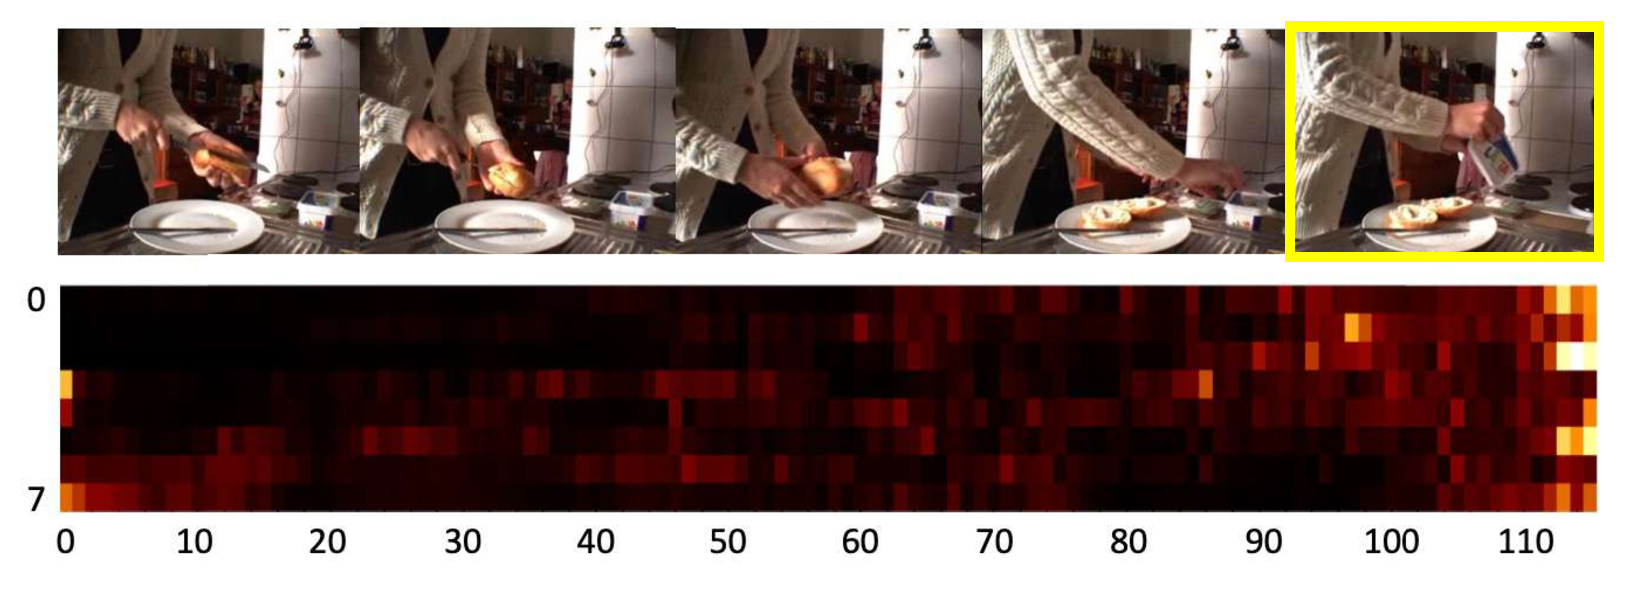
\includegraphics[width=\columnwidth]{Figures/pdf/sattn1_compressed.pdf}
    \counterwithin{figure}{section}
    \renewcommand\thefigure{S\arabic{figure}}
    \vspace{-5mm}
    \caption{Activity: Sandwich}
    \label{fig:s4a}
    \end{subfigure}
    
    \vspace{3mm}
    
    \begin{subfigure}[t]{0.75\linewidth}
    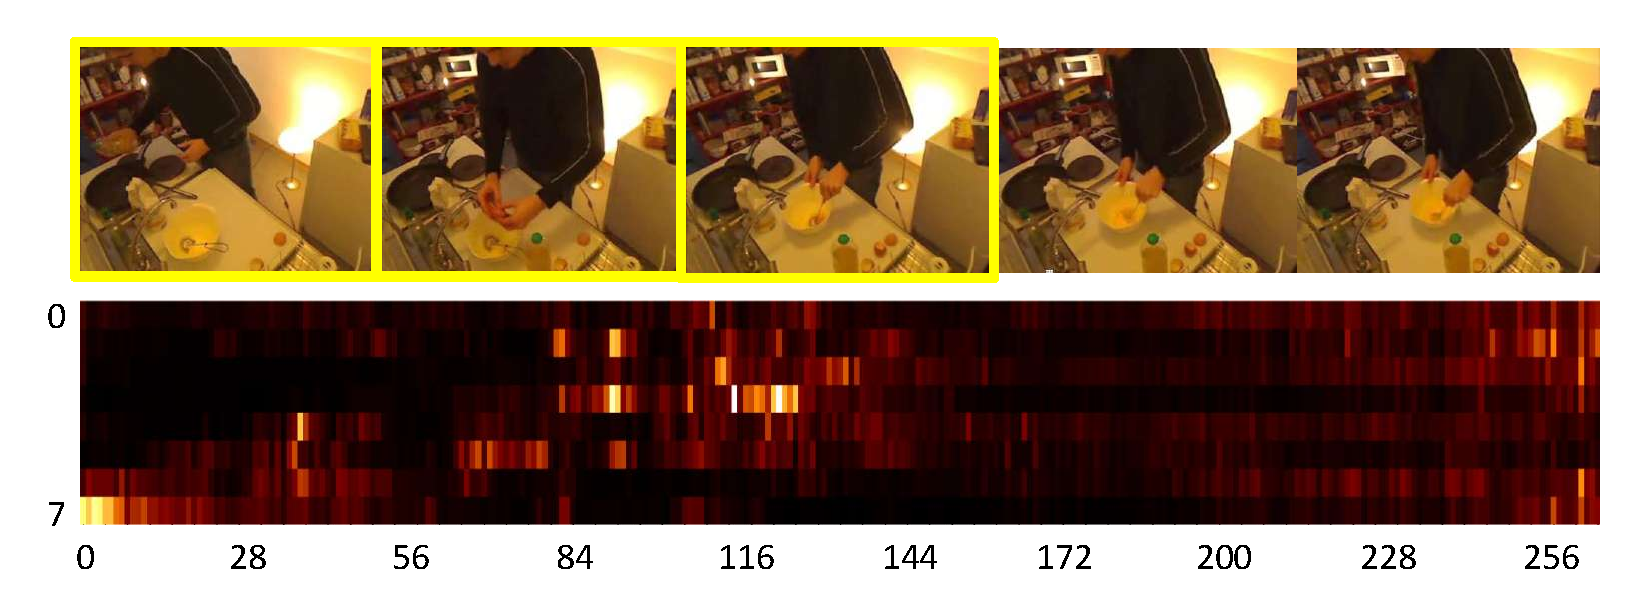
\includegraphics[width=\columnwidth]{Figures/pdf/sattn2_compressed.pdf}
    \counterwithin{figure}{section}
    \renewcommand\thefigure{S\arabic{figure}}
    \vspace{-6mm}
    \caption{Activity: Scramble egg}
    \label{fig:s4b}
    \end{subfigure}
    
    \vspace{3mm}
    
    \begin{subfigure}[t]{0.75\linewidth}
    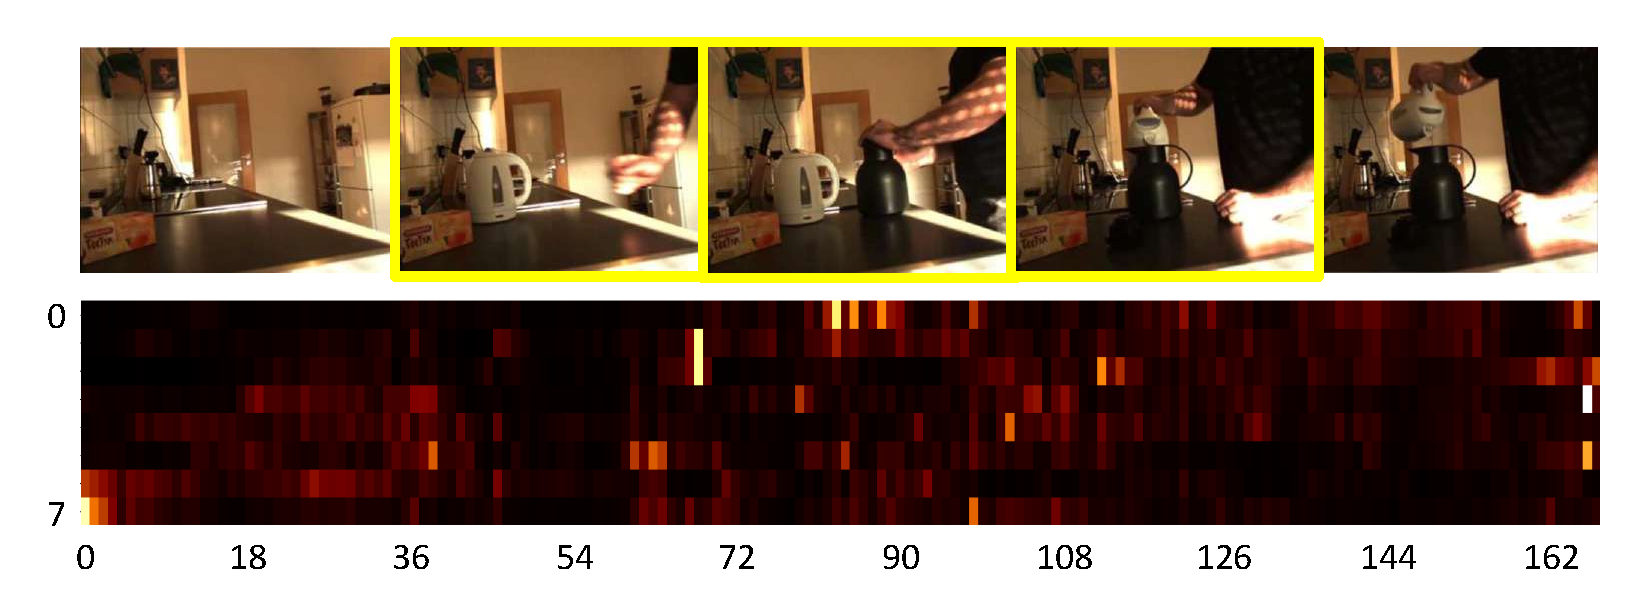
\includegraphics[width=\columnwidth]{Figures/pdf/sattn4_compressed.pdf}
    \counterwithin{figure}{section}
    \renewcommand\thefigure{S\arabic{figure}}
    \vspace{-6mm}
    \caption{Activity: Tea}
    \label{fig:s4d}
    \end{subfigure}
    
    \vspace{3mm}
    
    \begin{subfigure}[t]{0.75\linewidth}
    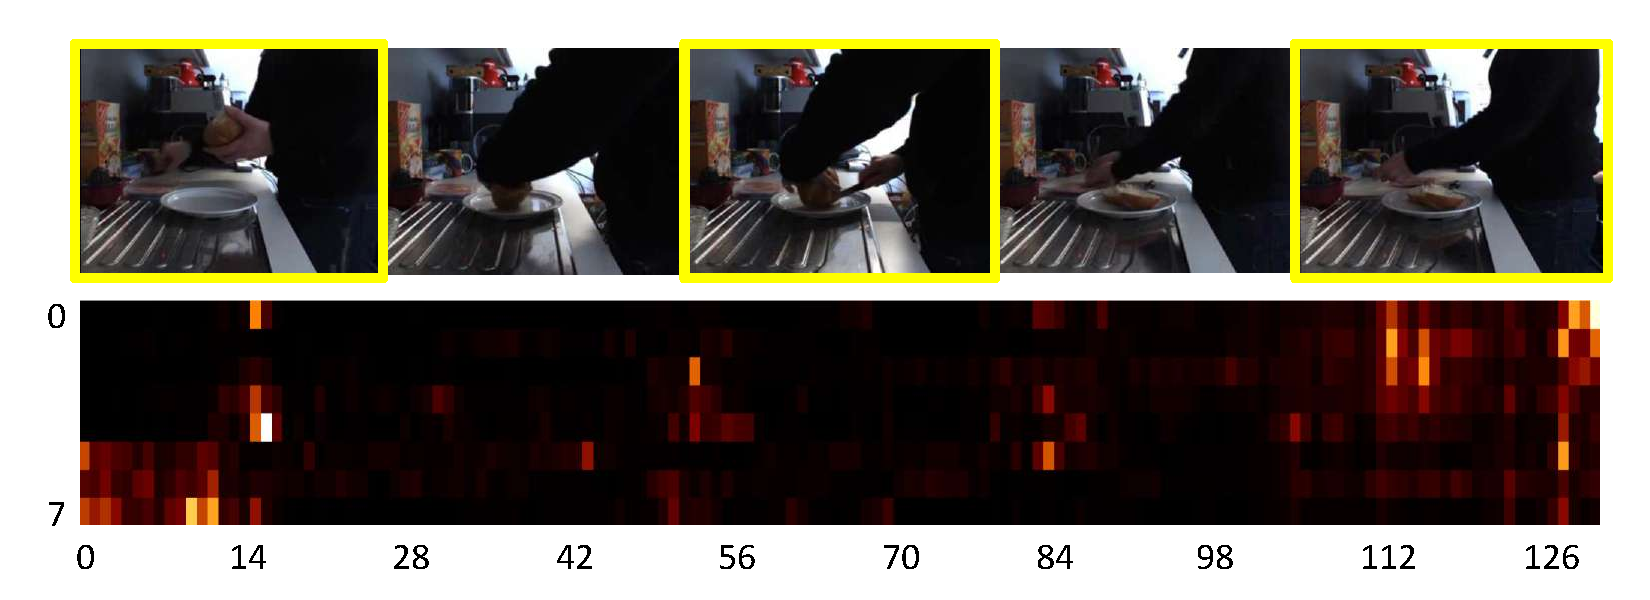
\includegraphics[width=\columnwidth]{Figures/pdf/sattn5_compressed.pdf}
    \counterwithin{figure}{section}
    \renewcommand\thefigure{S\arabic{figure}}
    \vspace{-6mm}
    \caption{Activity: Sandwich}
    \label{fig:s4e}
    \end{subfigure}
\counterwithin{figure}{section}
\renewcommand\thefigure{S\arabic{figure}}
\caption{\textbf{Cross-attention map visualization on Breakfast}. The vertical and horizontal axis indicates the decoder queries and observed frames, respectively. The brighter color indicates a higher attention score. RGB frames above the attention map are sampled uniformly from the video.
We emphasize the frames with high attention scores with yellow box and other frames are uniformly sampled. Best viewed in color.}
\vspace{-2mm}
 \label{fig:sup_attn}
\end{figure*}
\clearpage
\begin{figure*}[t]
    \centering
    \counterwithin{figure}{section}
    \renewcommand\thefigure{C\arabic{figure}}
    \begin{subfigure}[t]{0.95\linewidth}
    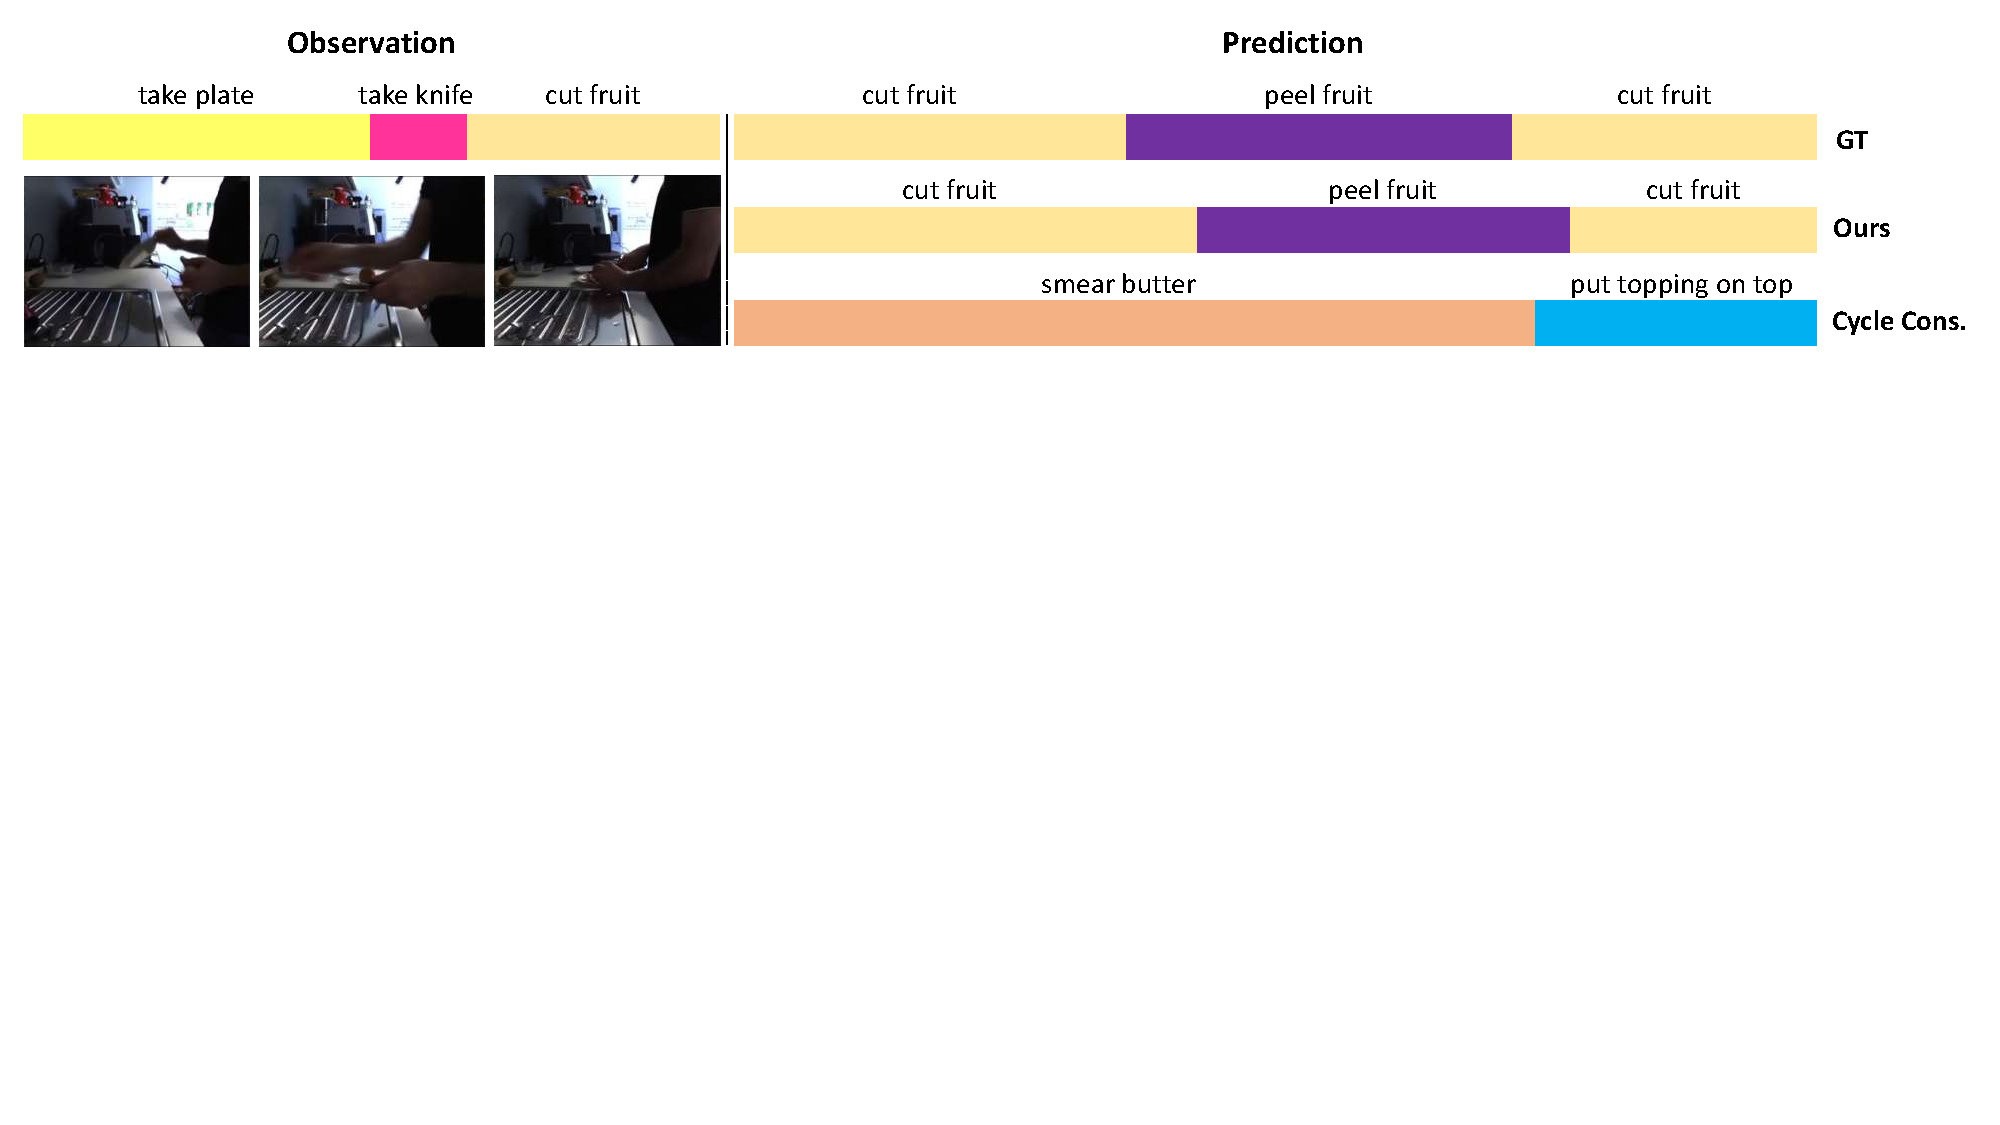
\includegraphics[width=\columnwidth]{Figures/pdf/squal4_compressed.pdf}
    \counterwithin{figure}{section}
    \renewcommand\thefigure{S\arabic{figure}}
    \vspace{-4mm}
    \caption{Activity: salad}
    \label{fig:s5a}
    \end{subfigure}
    
    \begin{subfigure}[t]{0.95\linewidth}
    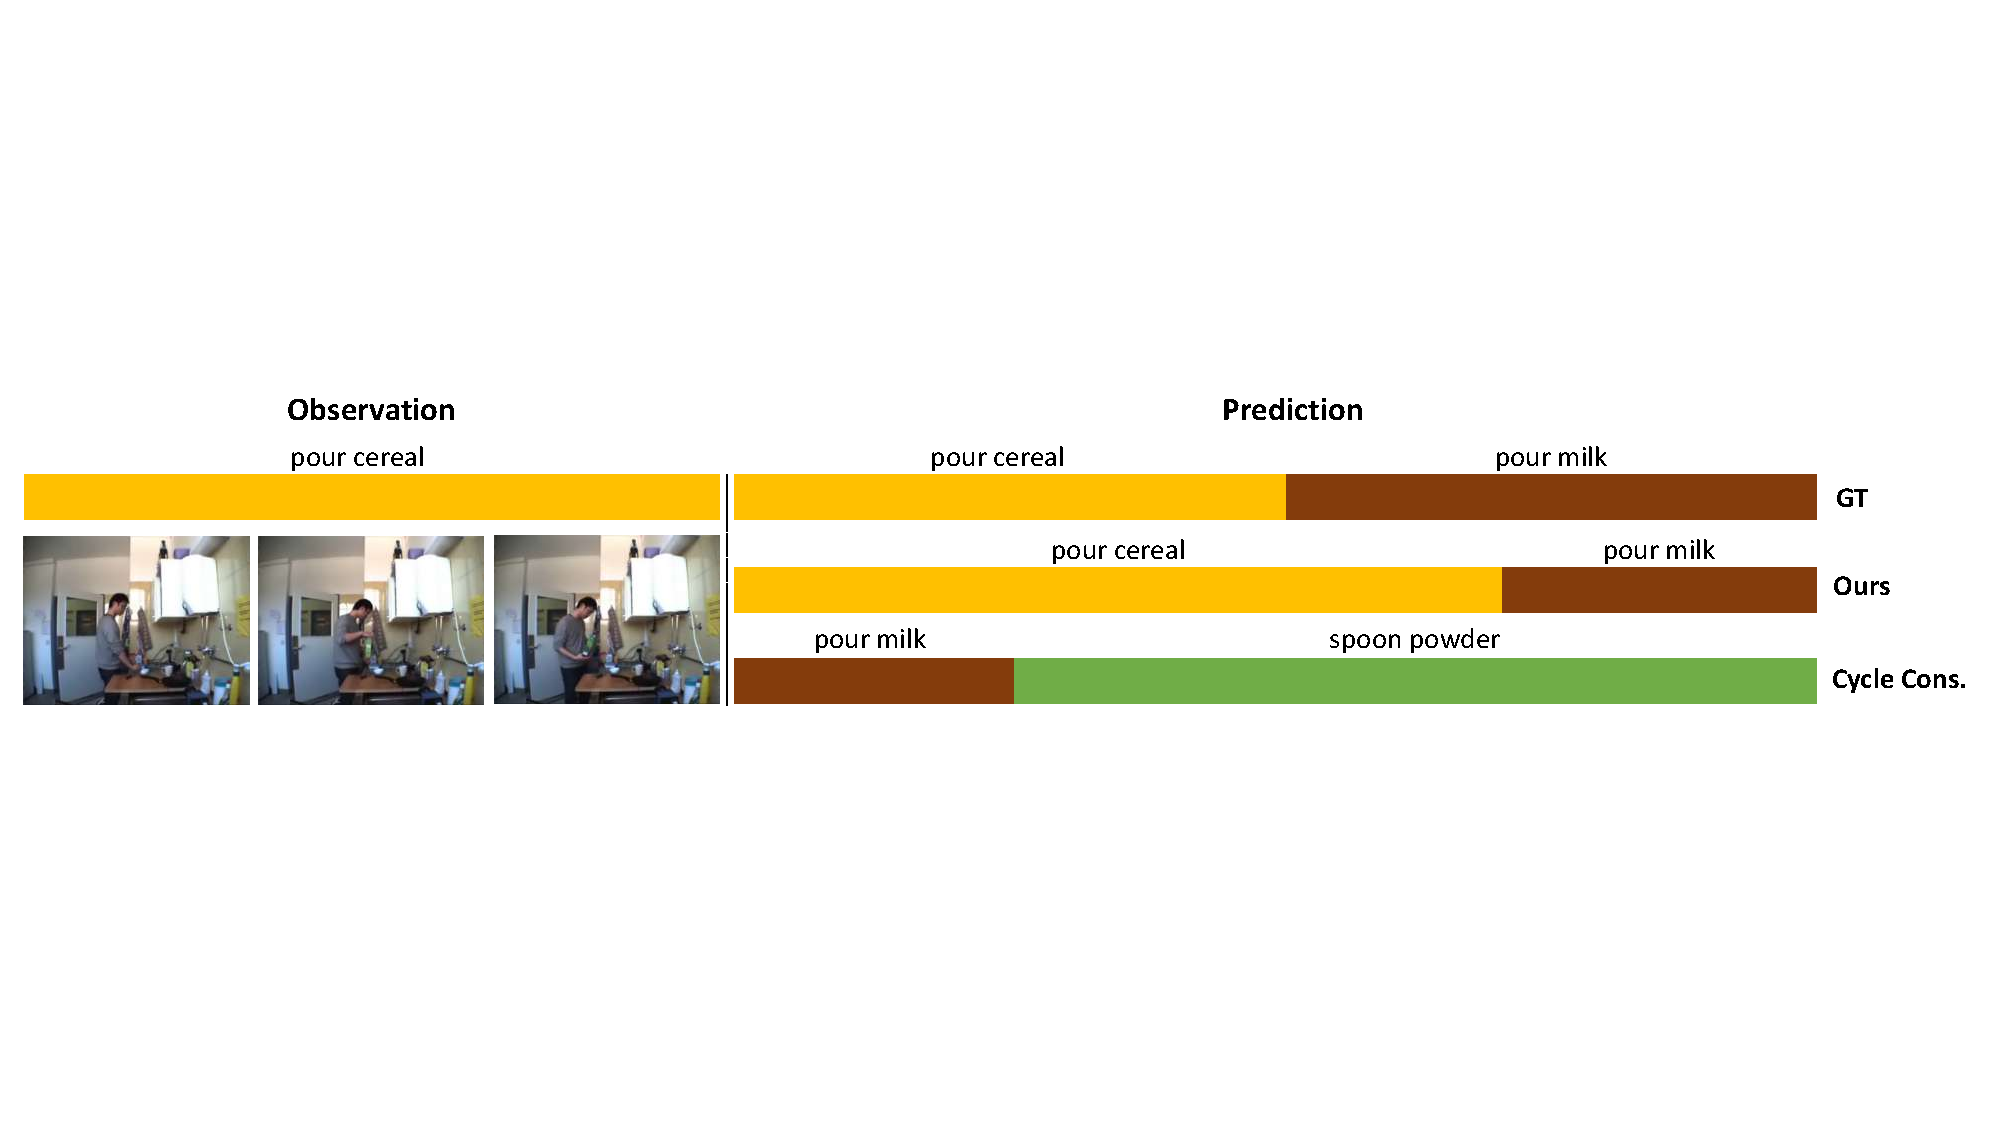
\includegraphics[width=\columnwidth]{Figures/pdf/squal2_compressed.pdf}
    \counterwithin{figure}{section}
    \renewcommand\thefigure{S\arabic{figure}}
    \vspace{-4mm}
    \caption{Activity: cereal}
    \label{fig:s5b}
    \end{subfigure}

    \begin{subfigure}[t]{0.95\linewidth}
    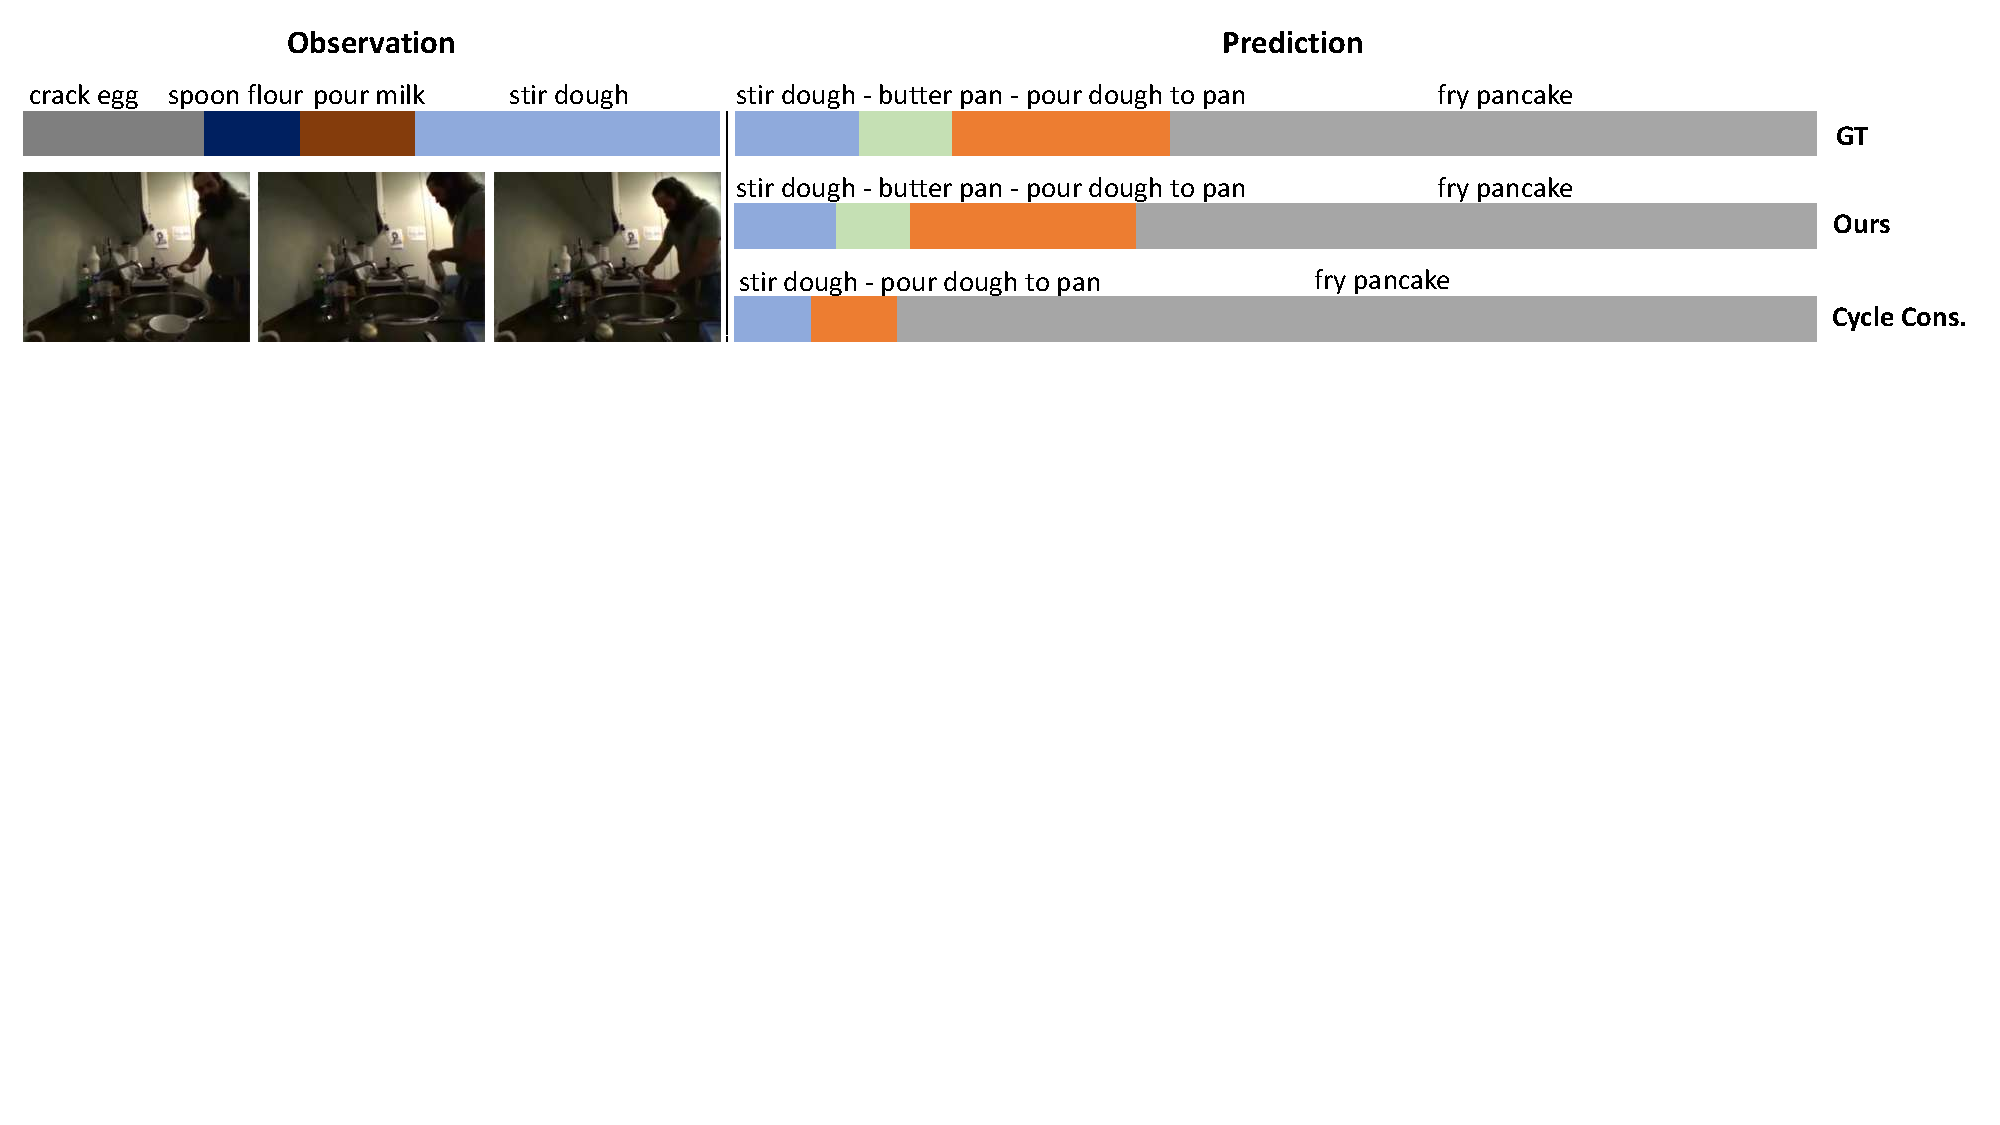
\includegraphics[width=\columnwidth]{Figures/pdf/squal1_compressed.pdf}
    \counterwithin{figure}{section}
    \renewcommand\thefigure{S\arabic{figure}}
    \vspace{-4mm}
    \caption{Activity: pancake}
    \label{fig:s5c}
    \end{subfigure}
    
    \begin{subfigure}[t]{0.95\linewidth}
    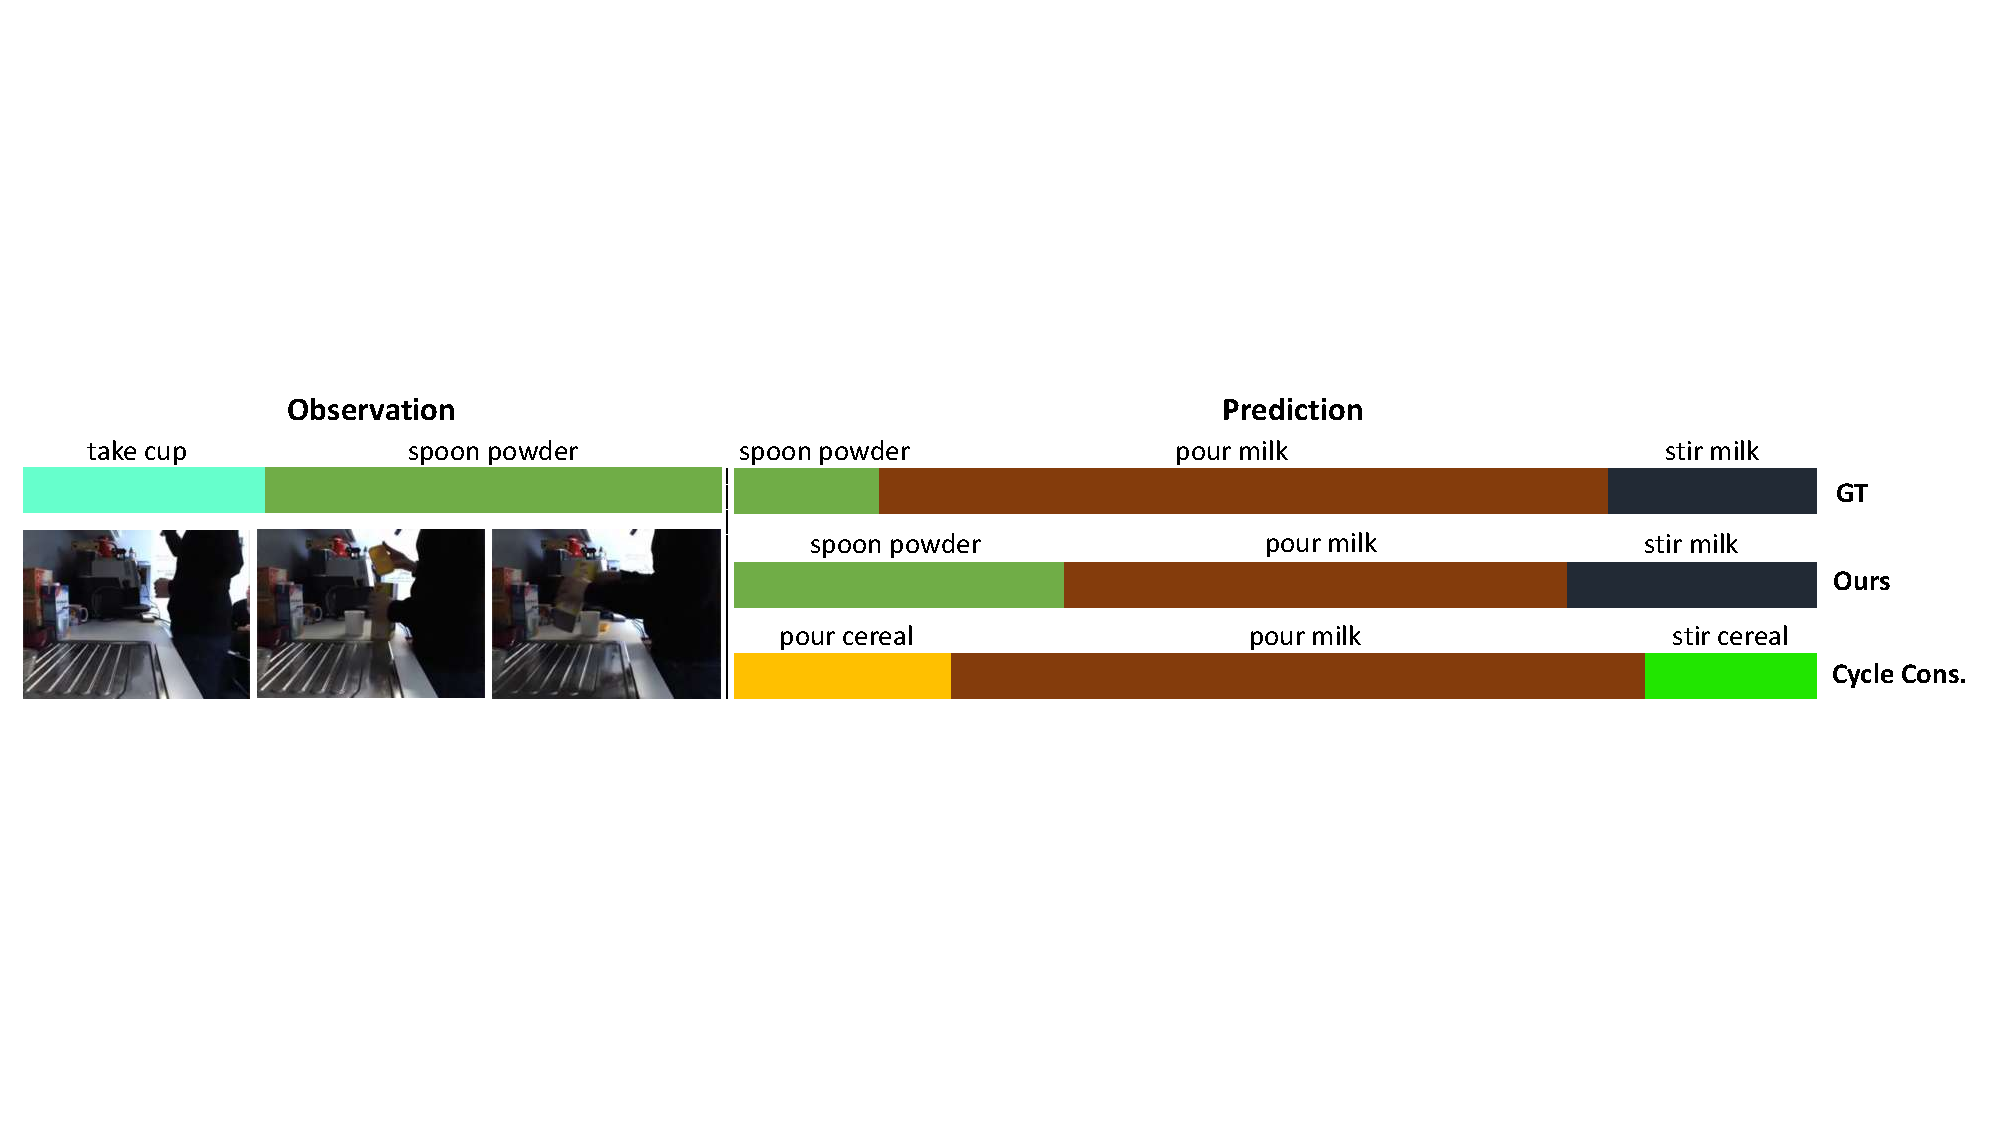
\includegraphics[width=\columnwidth]{Figures/pdf/squal5_compressed.pdf}
    \counterwithin{figure}{section}
    \renewcommand\thefigure{S\arabic{figure}}
    \vspace{-4mm}
    \caption{Activity: milk}
    \label{fig:s5d}
    \end{subfigure}
    
    \begin{subfigure}[t]{0.95\linewidth}
    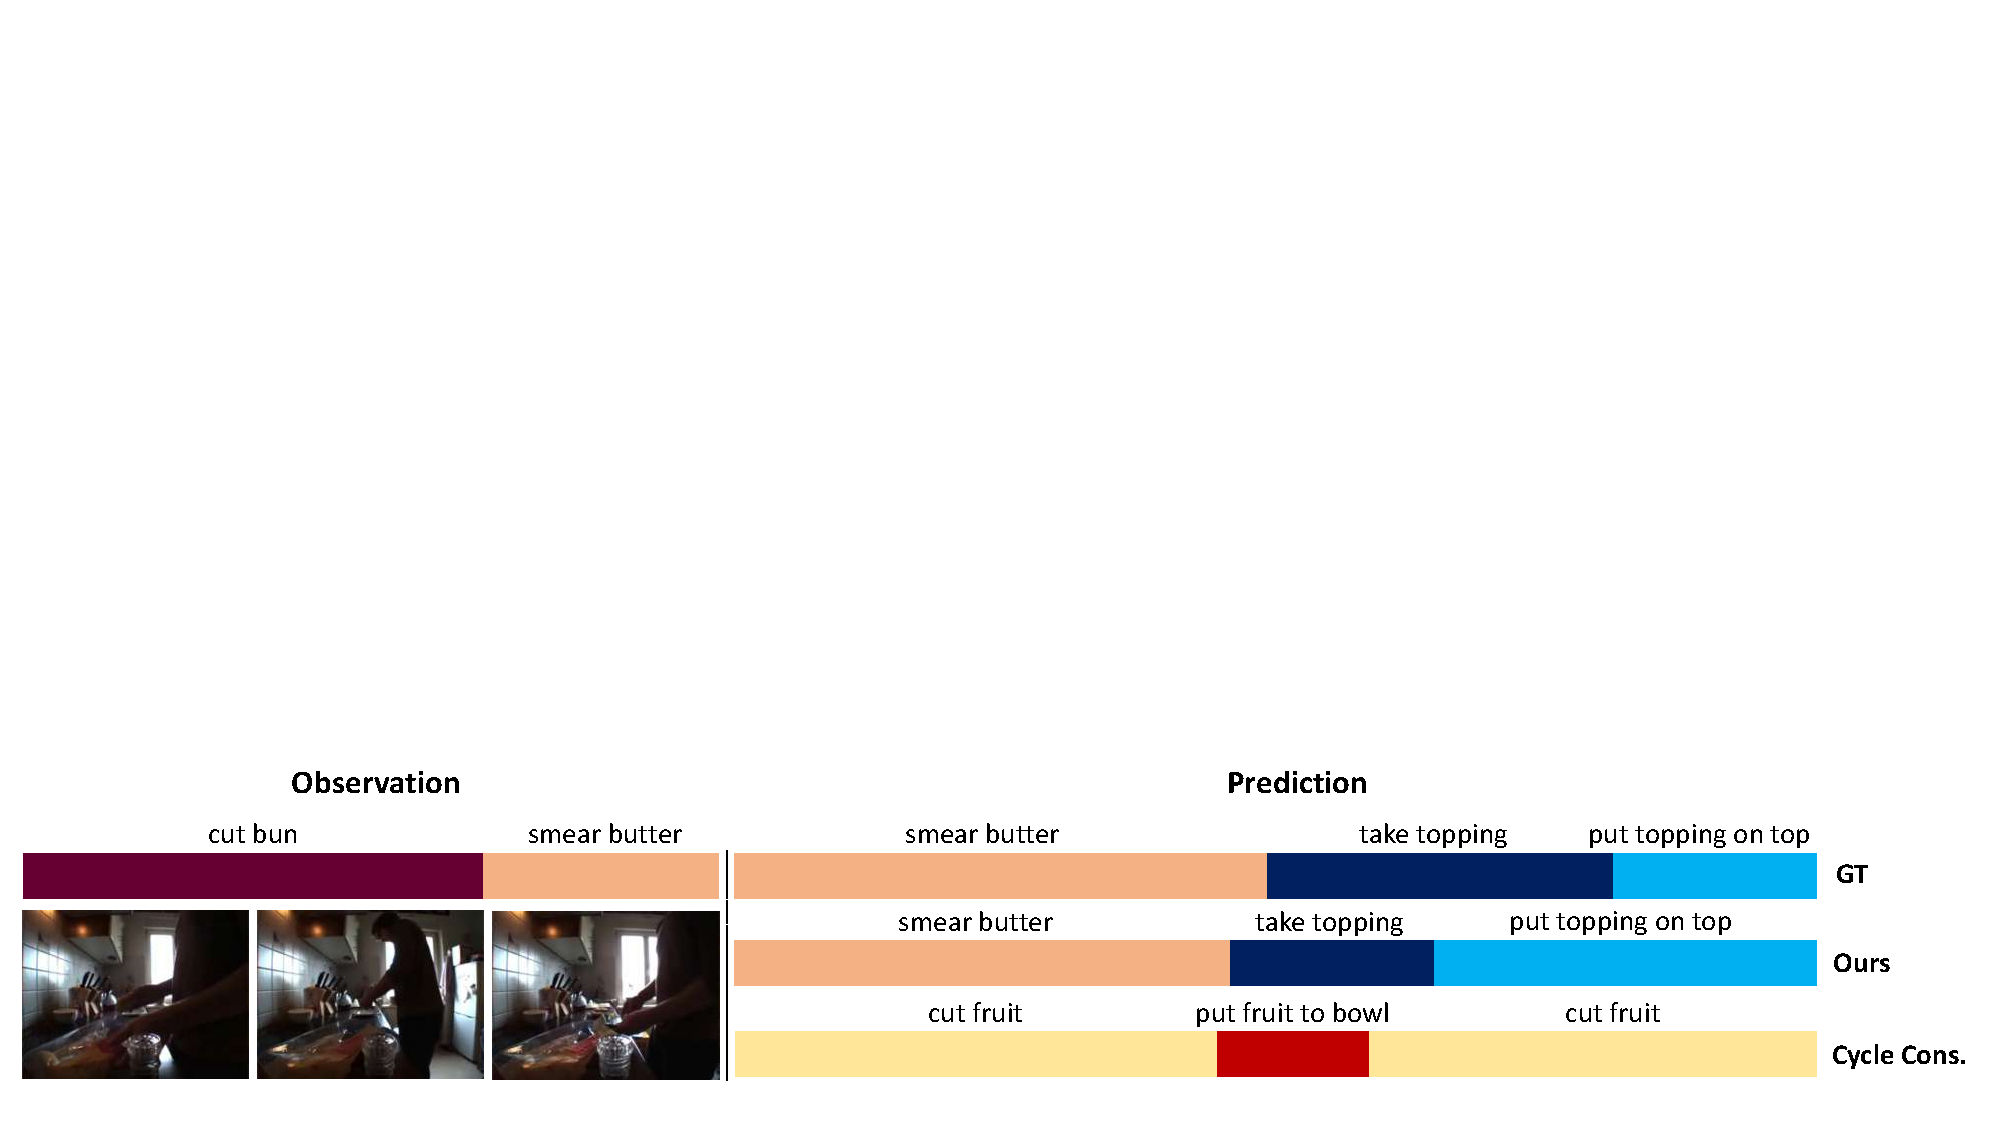
\includegraphics[width=\columnwidth]{Figures/pdf/squal3_compressed.pdf}
    \counterwithin{figure}{section}
    \renewcommand\thefigure{S\arabic{figure}}
    \vspace{-4mm}
    \caption{Activity: pancake}
    \label{fig:s5e}
    \end{subfigure}
\vspace{-2mm}
\counterwithin{figure}{section}
\renewcommand\thefigure{S\arabic{figure}}
\caption{\textbf{Qualitative results on Breakfast}. Each subfigure visualizes the ground truth label and the prediction results of the \ours and cycle consistency model proposed from Farha~\etal~\cite{farha2020long}. We set $ \alpha $ as 0.3 and $ \beta $ as 0.5 in this experiment. We decode action labels and durations to the frame-wise action classes. Each color in the color bar indicates an action label written above. Best viewed in color.}
\vspace{40mm}
 \label{fig:sup_qual}
\end{figure*}
\vspace{40mm}
